\section{Case Studies}

We have developed an open-source tool dReach using OCaml to perform $\delta$-complete reachability analysis for hybrid systems. dReach is built upon our SMT solver dReal \citep{dreal} that implements a $\delta$-complete decision procedure. All the experiments reported below were done using a machine with two Intel Xeon E5-2650 2.00GHz processors and 64GB RAM.

\subsection{Hormone therapy for prostate cancer}
Prostate cancer is the second leading cause of cancer-related deaths among men in United States \citep{cancerstat}. Hormone therapy in the form of androgen deprivation has been a cornerstone of the management of advanced prostate cancer for several decades. However, controversy remains regarding its optimum application \citep{nru}. Continuous androgen suppression (CAS) therapy has many side effects including anemia, osteoporosis, impotence, etc. Further, most patients experience a relapse after a median duration of 18-24 months of CAS treatment, due to the proliferation of androgen-independent (AI) cancer cells.

In order to reduce side effects of CAS and to delay the time to relapse, intermittent androgen suppression (IAS) was proposed aiming to limit the duration of androgen-poor conditions and avoid emergence of AI cells \citep{bruchovsky95}. In details, IAS therapy switches between on-treatment and off-treatment modes by monitoring the serum level of a tumor marker called prostate-specific antigen (PSA):  (i) when the PSA level decreases and reaches a lower threshold value $r_0$, androgen suppression is suspended; (ii) when the PSA level increases and reaches a upper threshold value $r_1$, androgen suppression is resumed by the administration of medical agents.

Recent clinical phase II and III trials confirm that IAS has significant advantages in terms of quality of life and cost. However, with respect to time to relapse and cancer-specific survival, the clinical trials suggest that to what extent IAS is superior to CAS depends on the individual patient and the on- and off-treatment scheme \citep{bruchovsky06,bruchovsky07,book13}. Thus, a crucial unsolved problem is how to design a personalized treatment scheme for each individual to achieve maximum therapeutic efficacy.

To answer this question, mathematical models have been developed to study the dynamics of prostate cancer under androgen suppression \citep{jackson04,ideta08, hirata10,pnas11}. Recently, attempts have been made to computationally classify patients and obtain the optimal treatment scheme \citep{chaos10,suzuki10}. However, these results relied on simplifying nonlinear hybrid dynamical systems to more manageable versions such as piecewise linear models \citep{chaos10} and piecewise affine systems \citep{suzuki10}. In this section, we show that our $\delta$-decision based parameter synthesis approach can help to design personalized treatment scheme based on nonlinear hybrid systems with arbitrary computable real functions. Here we focus on the hybrid model presented by \cite{ideta08}, which describes the growth of a prostate tumor as the dynamics of a mixed population of androgen-dependent (AD) and androgen-independent (AI) cells. 

The model has two modes which are shown in Figure \ref{pmodel}. $x(t)$, $y(t)$, and $z(t)$ represent the population of AD cells, the population of AI cells, and the serum androgen concentration, respectively. The growth dynamics of AD and AI cells are governed by their proliferation rate, apoptosis rate and mutation rate from AD to AI phenotype, depending on androgen concentration $z(t)$. The PSA level $v$ (ng ml$^{-1}$) is defined as $v(t)=x(t)+y(t)$. The treatment is suspended or restarted according to the value of $v$ and ${dv}/{dt}$. In mode $2$ (off-treatment), the androgen concentration is maintained at the normal level $z_0$ by homeostasis. In mode $1$ (on-treatment), the androgen is cleared at a rate $1/\tau$. Table \ref{prostate} lists the values of model parameters.

\begin{figure}[htb]
\centering
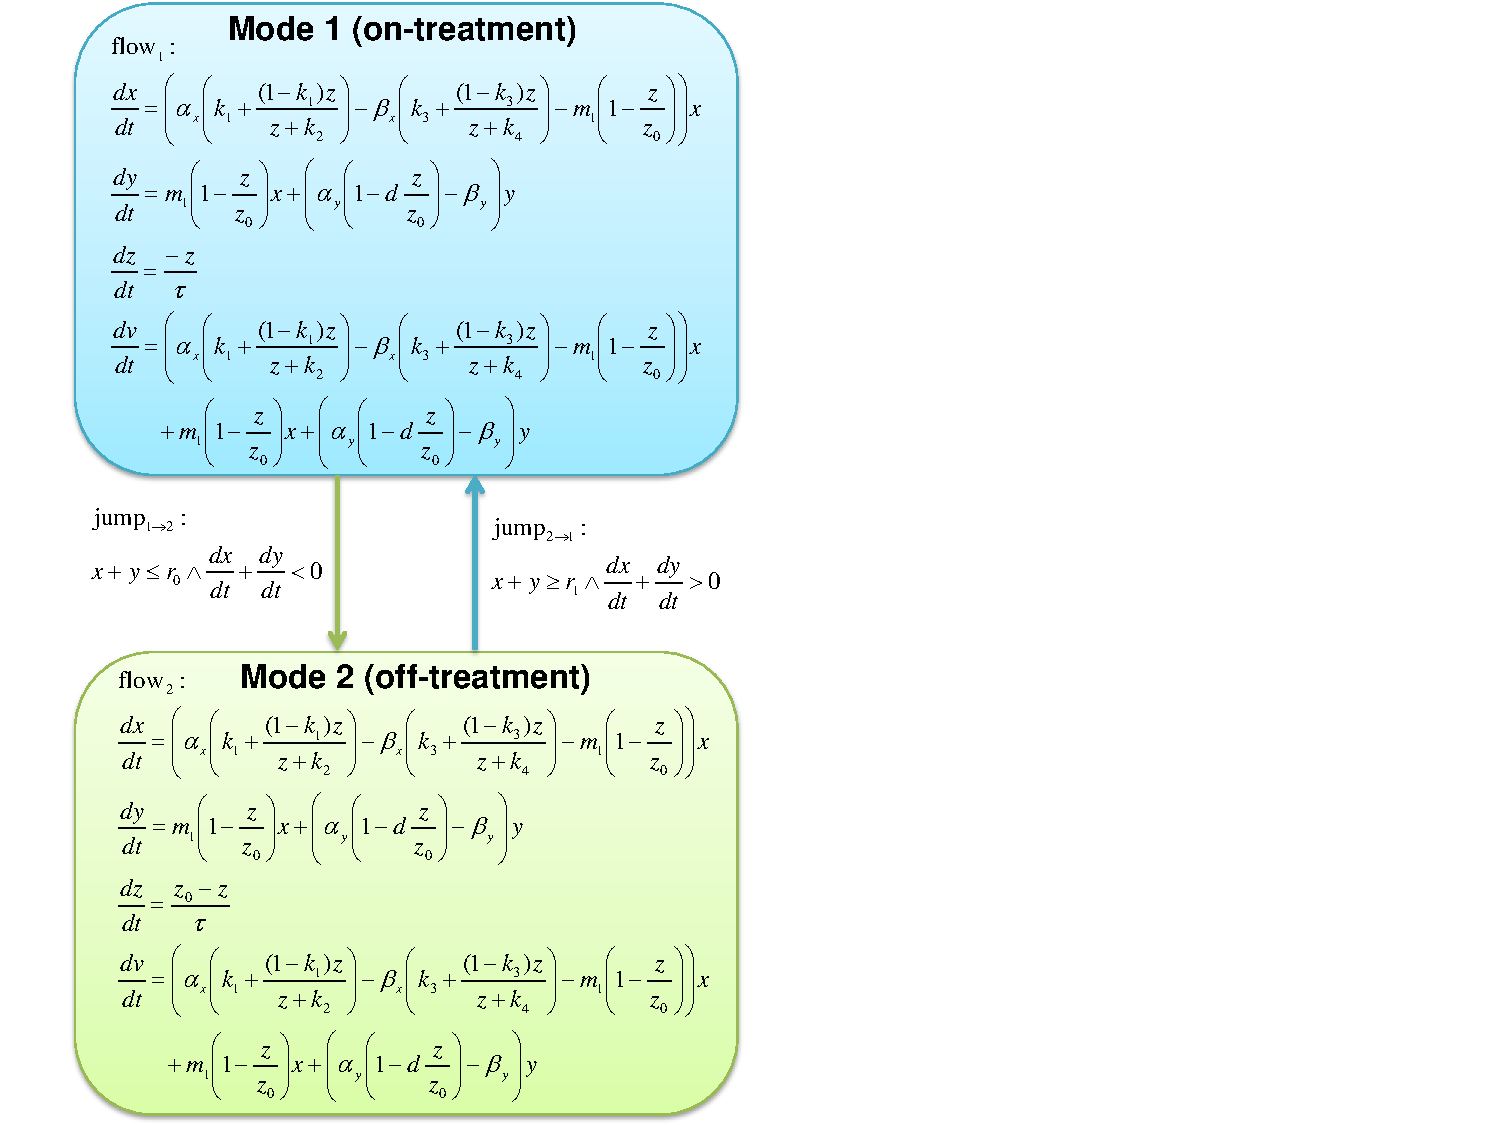
\includegraphics[scale=0.5]{fig-prostate}
\caption{The prostate cancer treatment model.}
\label{pmodel}
 \vspace{-0.7cm}
\end{figure}



\begin{table}[htb]
\processtable{Prostate cancer model parameter values\label{prostate}}
{\begin{tabular}{lll}\toprule
Parameter  & Bone metastasis & Lymph node metastasis  \\\midrule
$\alpha_x$ & 0.0204 d$^{-1}$ & 0.0168 d$^{-1}$  \\
$\alpha_y$ & 0.0242 d$^{-1}$ & 0.0277 d$^{-1}$  \\
$\beta_x$  & 0.0076 d$^{-1}$ & 0.0085 d$^{-1}$  \\
$\beta_y$  & 0.0168 d$^{-1}$ & 0.0222 d$^{-1}$  \\
$k_1$     & 0.0 nM & 0.0 nM \\
$k_2$     & 2.0 & 2.0  \\
$k_3$     & 8.0 nM & 8.0 nM \\
$k_4$     & 0.5 & 0.5  \\
$m_1$     & 0.00005 d$^{-1}$ & 0.00005 d$^{-1}$  \\
$z_0$     & 20.0 nM & 20.0 nM  \\
$\tau$     & 62.5 d & 62.5 d \\
\botrule
\end{tabular}}{}
 \vspace{-0.7cm}
\end{table}

\subsubsection{Model selection}
Based on different assumptions of the proliferation dynamics of AI cells, the above model has three variations, denoted as $H_1$, $H_2$, and $H_3$, which are discriminated by the value of $d$, i.e.:
\begin{itemize}
\item $H_1$: AI cells grow at the constant rate independent of the androgen level ($d=0$)\\
\item $H_2$: AI cells do not grow when the androgen level is normal ($d=1-\beta_2/\alpha_2$)\\
\item $H_3$: AI cells decrease when the androgen level is normal ($d=1)$
\end{itemize}

In order to perform model selection using $\delta$-decision procedures, we specified the cancer relapse as a state with ``$v>30$'', since the PSA level $v$ reflects the total number of tumor cells. We then checked whether each of the model candidates can reach a relapse state within a bounded time of $1000$ days. Here the treatment scheme threshold parameters were fixed as $r_0=4$ (ng ml$^{-1}$) and $r_1=10$ (ng ml$^{-1}$). The range of the initial concentration of androgen was given as $[10, 20]$ (nM).

Given the invariant $v \in [0,30]$, $H_1$ and $H_2$ are unable to reach a state with $t=1000$. In other words, $H_1$ and $H_2$ will always lead to cancer relapse state no matter which initial androgen concentration was chosen. This is conflict with the clinical observations by \cite{bruchovsky06,bruchovsky07}. In contrast, $H_3$ is able to avoid the relapse state and reproduce the experimental observation (see Figure \ref{prostate-fig1}). Thus, we completed the model selection process by ruling out $H_1$ and $H_2$ and choose $H_3$ for further analysis.


\begin{figure}[htb]
\centering
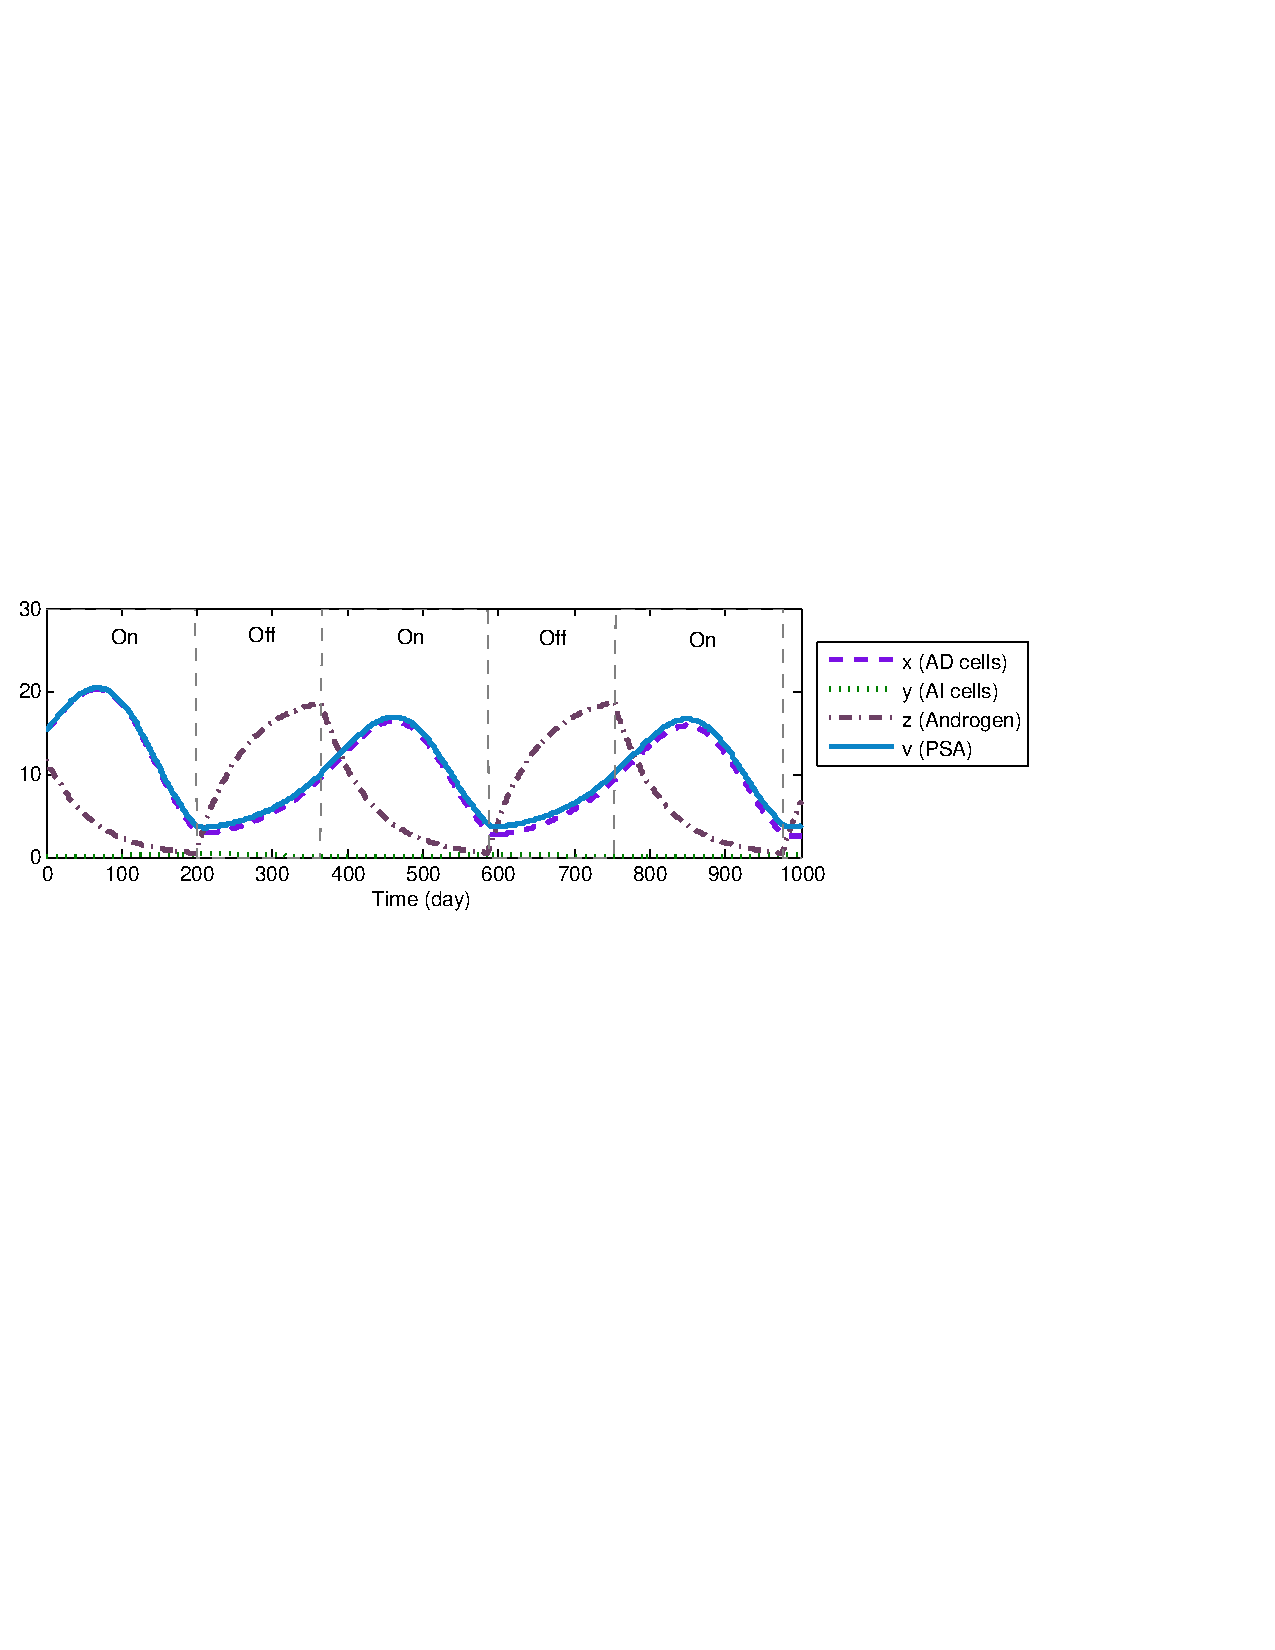
\includegraphics[scale=0.5]{fig-prostatetraj}
\caption{Simulated time profiles of $H_3$ model.}
\label{prostate-fig1}
 \vspace{-0.7cm}
\end{figure}

\subsubsection{Personalized therapy design}
We next apply our parameter synthesis method to selecting suitable therapy and designing personalized treatment scheme for individual patients. Note that the parameter values in Table \ref{prostate} were estimated from clinical data of hundreds of patients \citep{bruchovsky07}. Among patients, the values of some parameters vary, which causes the variability in responsiveness to hormone therapy. We select a set of ``personalized parameters'' including $\alpha_y$ (the proliferation rate of AI cells), $\beta_y$ (the apoptosis rate of AI cells), $m_1$ (the mutation rate from AD to AI cells), and $z(0)$ (the initial androgen level). The values of these parameters can be either experimentally measured \citep{berges95} or computationally determined from PSA time serials data \citep{hirata10}.

Figure \ref{patients}(a-c) illustrates the PSA dynamics of $3$ patients with different personalized parameters under the same IAS treatment scheme ($r_0=4$, $r_1=10$). IAS prevents the relapse for Patient\#1 and delays the relapse for Patient\#2, but does not help Patient\#3. Figure \ref{patients}(d) shows that, by modifying the IAS scheduling parameters $r_0$ and $r_1$, the relapse of Patient\#3 can be avoided or delayed. Thus, we can formulate the personalized therapy design problem as a parameter synthesis procedure: (i) fill in parameter values of a patient to $H_3$; (ii) set the ranges of scheduling parameters as $r_0 \in [0,8)$ (nM) and $r_1 \in [8,15]$; (iii) check if $H_3$ can reach a state with $t=1000$ given the invariant $v \in [0,30]$ (i.e. no relapse). If the $\delta$-decision procedure returns $\mathsf{False}$, it means that androgen suppression therapy is not suitable for the patient. Otherwise, a treatment scheme containing feasible values of $r_0$ and $r_1$ will be returned, which could prevent or delay the relapse of the patient. Note that if $r_0=0$ is returned, it refers to the CAS scheme.

\begin{figure}[htb]
\centering
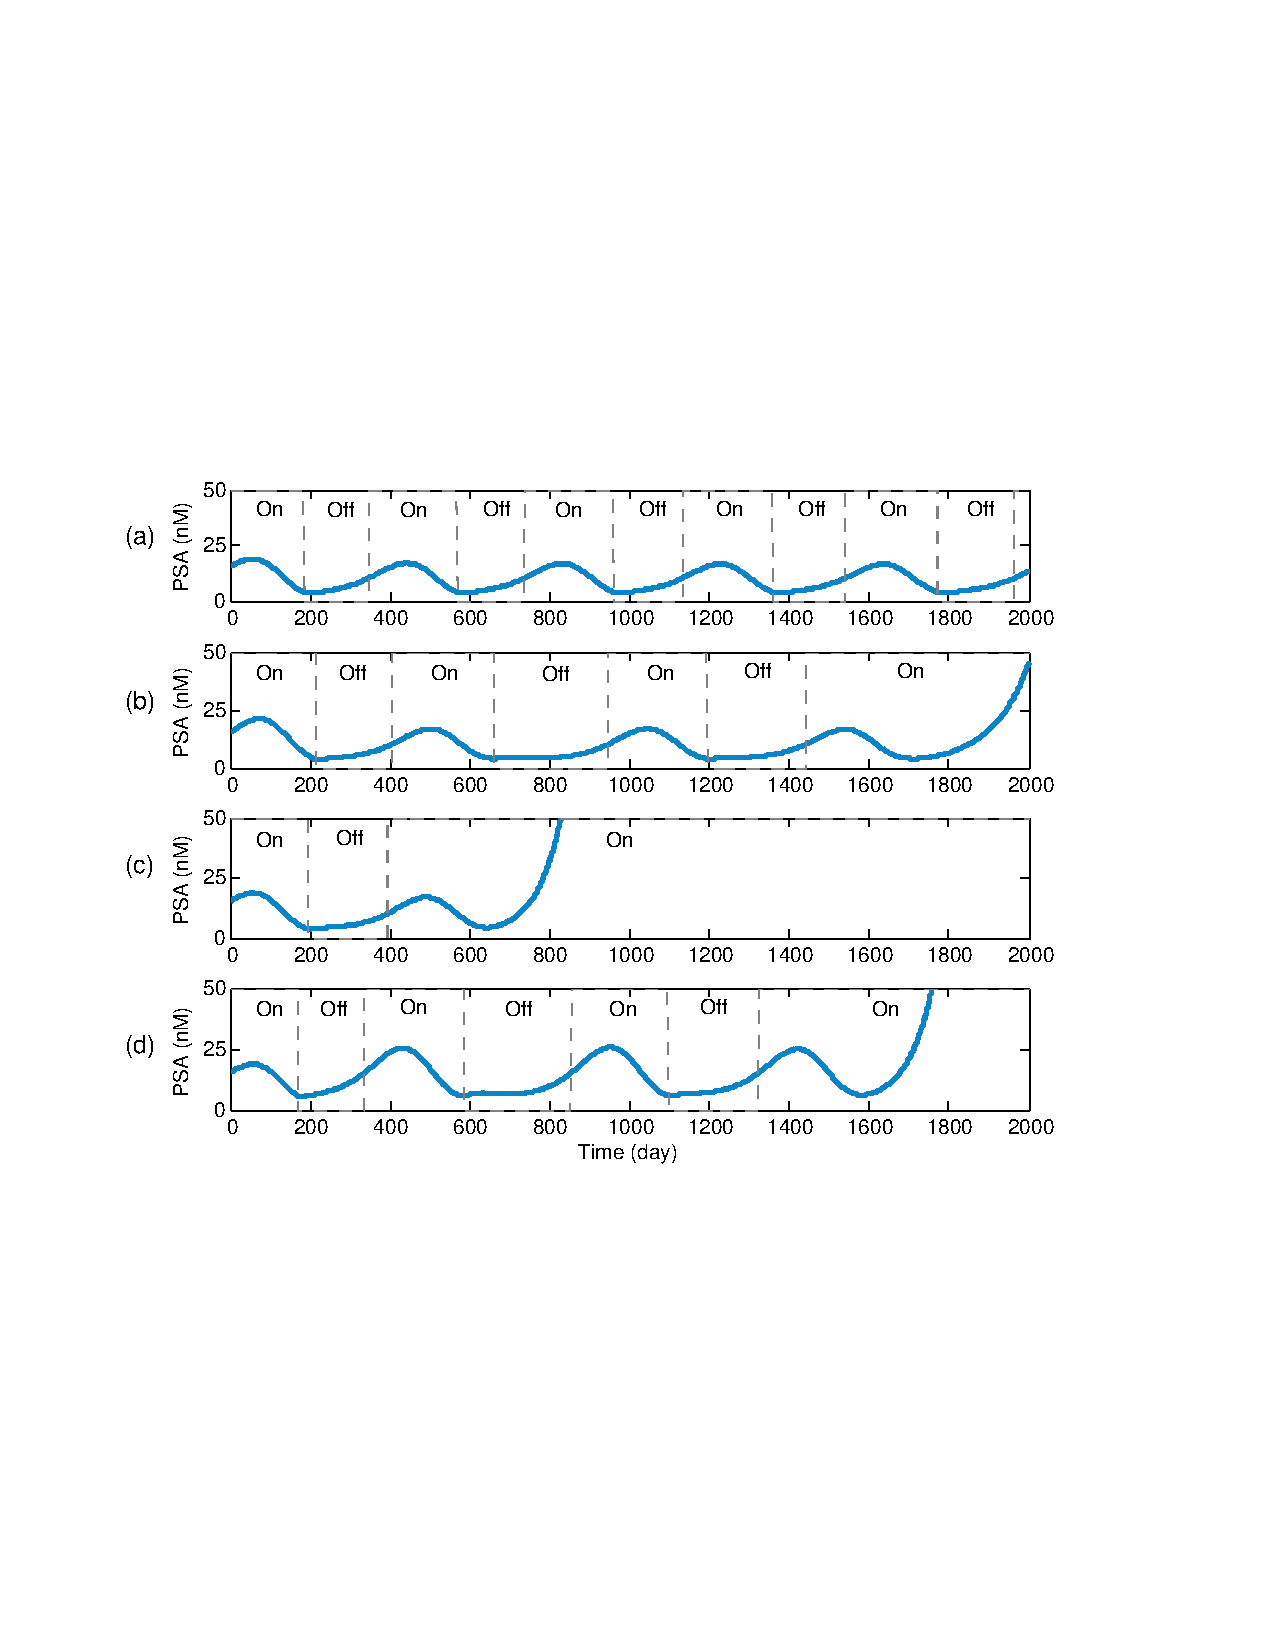
\includegraphics[scale=0.55]{fig-prostatetraj2}
\caption{Simulated PSA profiles of patients with different parameters. (a) Patient\#1: $\alpha_y=0.0242$, $\beta_y=0.0168$, $m_1=0.00005$, $z(0)=12$, $r_0=4$, $r_1=10$ (b) Patient\#2: $\alpha_y=0.24$, $\beta_y=0.13$, $z(0)=13$, $m_1=0.0001$, $r_0=4$, $r_1=10$ (c) Patient\#3: $\alpha_y=0.35$, $\beta_y=0.187$, $m_1=0.00005$, $z(0)=10$, $r_0=4$, $r_1=10$ (d) Patient\#3: $\alpha_y=0.035$, $\beta_y=0.187$, $m_1=0.00005$, $z(0)=10$, $r_0=6$, $r_1=15$.}
\label{patients}
 \vspace{-0.7cm}
\end{figure}


We tested our method on real patients data collected by \cite{bruchovsky07}. The values of $\alpha_y$, $\beta_y$, $m_1$, and $z(0)$ for each selected patient were estimated by fitting the model to the PSA time serials data under the first $1.5$ cycles of IAS therapy (data available at http://www.nicholasbruchovsky.com/clinicalResearch.html). Table \ref{prostate2} summarized the suggested treatment scheme for selected patients. The in silico validation results are shown in Supplementary Materials.

\begin{table}[htb]
\processtable{Personalized hormone therapy scheme for selected patients\label{prostate2}}
{\begin{tabular}{llllll}\toprule
Patient ID  & $\alpha_y$  & $\beta_y$ & $m_1$ & $z(0)$ & Suggested scheme  \\\midrule
\#8 & 0.025 & 0.021  & 3.0E-5 & 8.23 & $r_0=5.0$, $r_1=11.2$ \\
\#10 & 0.019 & 0.009  & 5.9E-5 & 9.44 & $r_0=4.1$, $r_1=9.4$ \\
\#45 & 0.012  & 0.041  & 1.0E-5 & 12.61 & $r_0=3.8$, $r_1=12.2$ \\
\#97 & 0.031  & 0.015  & 2.3E-5 & 10.61 & $-$ \\
\botrule
\end{tabular}}{}
 \vspace{-0.7cm}
\end{table}

\begin{figure*}[t]
\centering
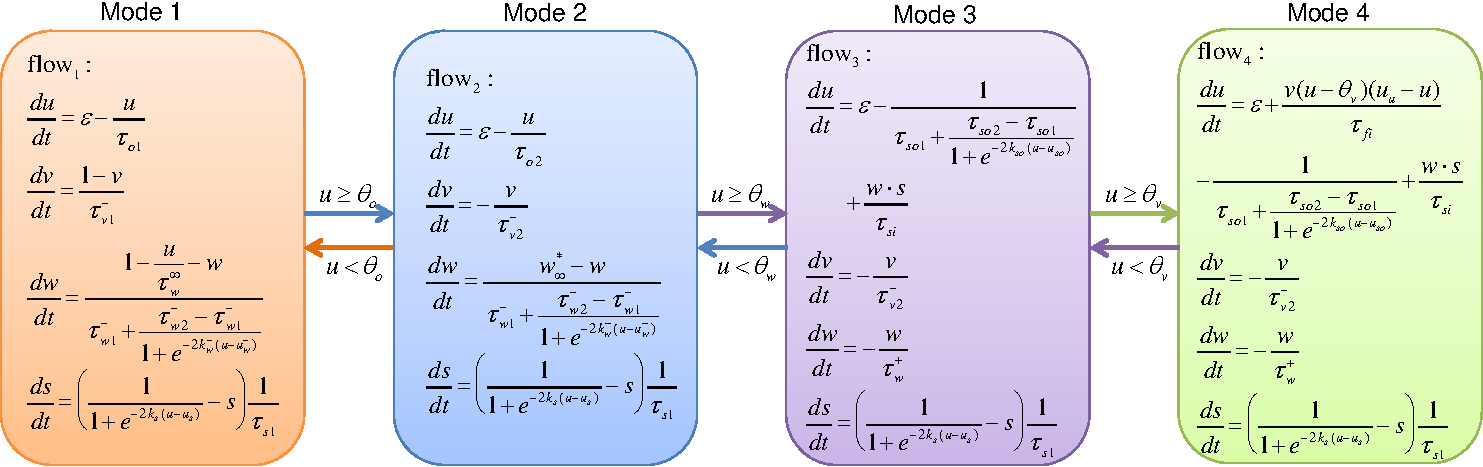
\includegraphics[scale=0.65]{fig-cardiac}
\caption{The minimal resistor model of cardiac cells.}
\label{mrm}
 \vspace{-0.7cm}
\end{figure*}


\subsection{Parameter identification for cardiac disorders}

Mathematical modeling the dynamics of cardiac cells is important in understanding the mechanisms of cardiac disorders. \cite{orovio08} has developed an extremely versatile electrical model for cardiac cells, referred as minimum resistor model (MRM), which reproduces experimentally measured characteristics of human ventricular cell dynamics. Identifying the parameter ranges for which the MRM accurately reproduces cardiac abnormalities will benefit the development of the treatment of cardiac disorders. For instance, improper functioning of the cardiac cell ionic channels may cause the cells to lose excitability. Unexcitable cells can induce ventricular tachycardia or fibrillation by blocking propagating electrical waves. In order to identify parameter ranges for which cardiac cells loss excitability, \cite{grosu11} linearized and transformed MRM into a piecewise-multiaffine system called MHA so that parameters synthesis process can be performed using the method proposed in \cite{rovergene}. However, due the the simplification, MRM and MHA have different sets of parameters. In this section, we show how we identify MRM parameter ranges for cardiac disorders without the help of linear approximation.



MRM contains $4$ state variables and $26$ parameters. An action potential (AP) is a change in the cell's transmembrane potential $u$, as a response to an external stimulus (current) $\epsilon$. The flow of total currents is controlled by a fast channel gate $v$ and two slow gates $w$ and $s$. %Figure \ref{mrm} shows the $4$ modes associated with MRM. The parameter values can be found in Supplementary Materials.
%
%
%\begin{figure}[h]
%\centering
%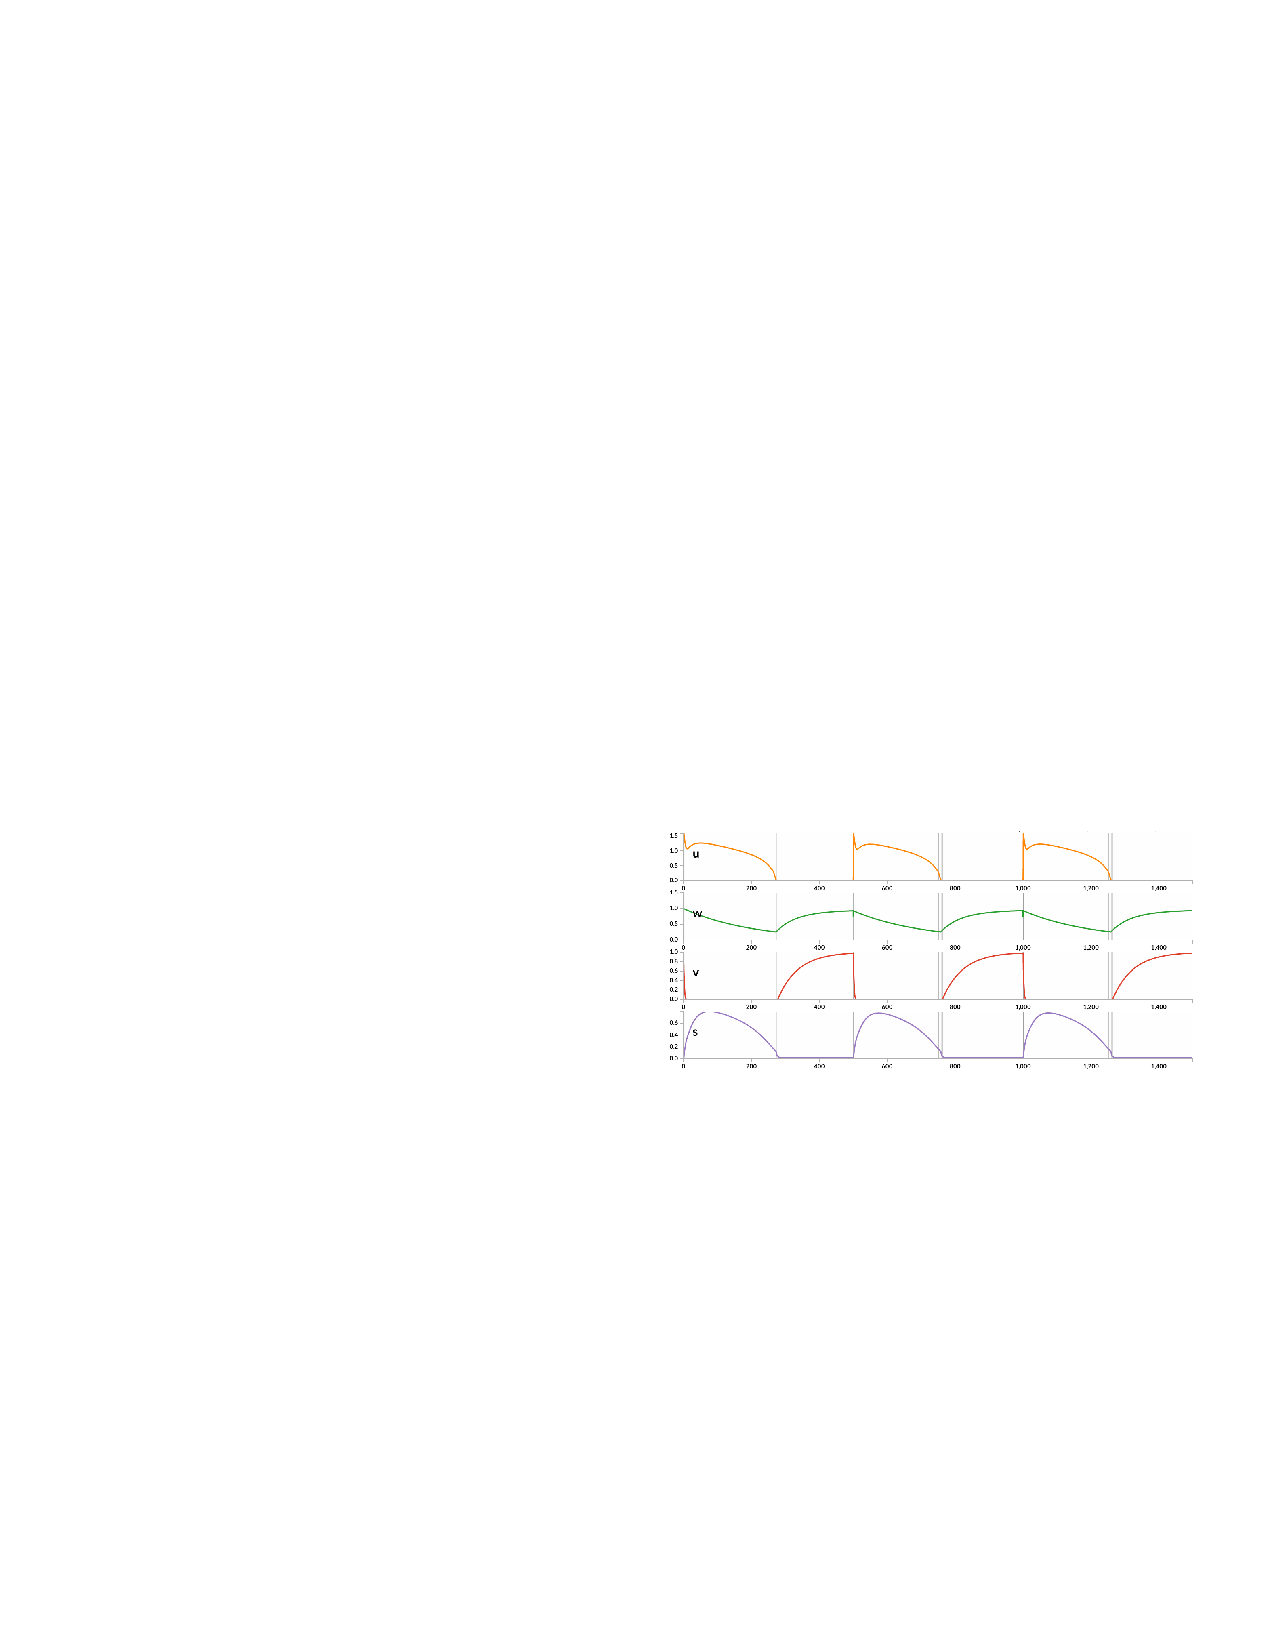
\includegraphics[scale=1]{fig-cardiactraj}
%\caption{The simulated time profile of MRM.}
%\label{ctrace}
% \vspace{-0.7cm}
%\end{figure}
%
In Mode $1$, gates $v$ and $w$ are open and gate $s$ is closed. The transmembrane potassium current causes the decay of $u$. The cell is resting and waiting for stimulation. We assume external stimulus $\epsilon$ equals to $1$ and lasts for $1$ millisecond. The stimulation causes $u$ increase which may trigger $\jump_{1 \rightarrow 2}: u \geq \theta_o$. In Mode 2, $v$ starts closing. The decay rate of $u$ changes. The systems will jump to Mode 3 if $u \geq \theta_w$. In Mode 3, $w$ is also closing. $u$ is governed by the potassium current and the calcium current. When $u \geq \theta_v$, Mode 4 can be reached which means a successful AP initiation. In Mode 4, $u$ reaches its peak due to the fast opening of sodium channel. The cardiac muscle contracts and $u$ starts decreasing. Figure \ref{ctrace} shows a witness trace computed by dReal when Mode 4 is reachable. The stimulus $\epsilon$ was reset every $500$ milliseconds.







When the system can not reach a state in Mode 4, the cardiac cell loses the excitability, which might lead to tachycardia and fibrillation. Starting with Mode 1, we then synthesized parameters using which the system will never go into Mode 4. We obtained the following results (see Supplementary Materials for more details):
$$\tau_{o1} \in (0,0.006)\vee \tau_{o2} \in (0,0.13)\vee 6.2 \cdot \tau_{so1} + \tau_{so2} \ge 9.9$$

The results suggest that when $\tau_{o1} \in (0, 0.006)$, the system will always stay in Mode 1. When $\tau_{o2} \in (0, 0.13)$, a state in Mode 3 can not be reached. Furthermore, whether the system can jump from Mode 3 to Mode 4 depends on the interplay between $\tau_{so1}$ and $\tau_{so2}$.  Figure \ref{cresults} visualizes these results by showing the simulated time profiles with different parameter values.



\begin{figure}[h]
\centering
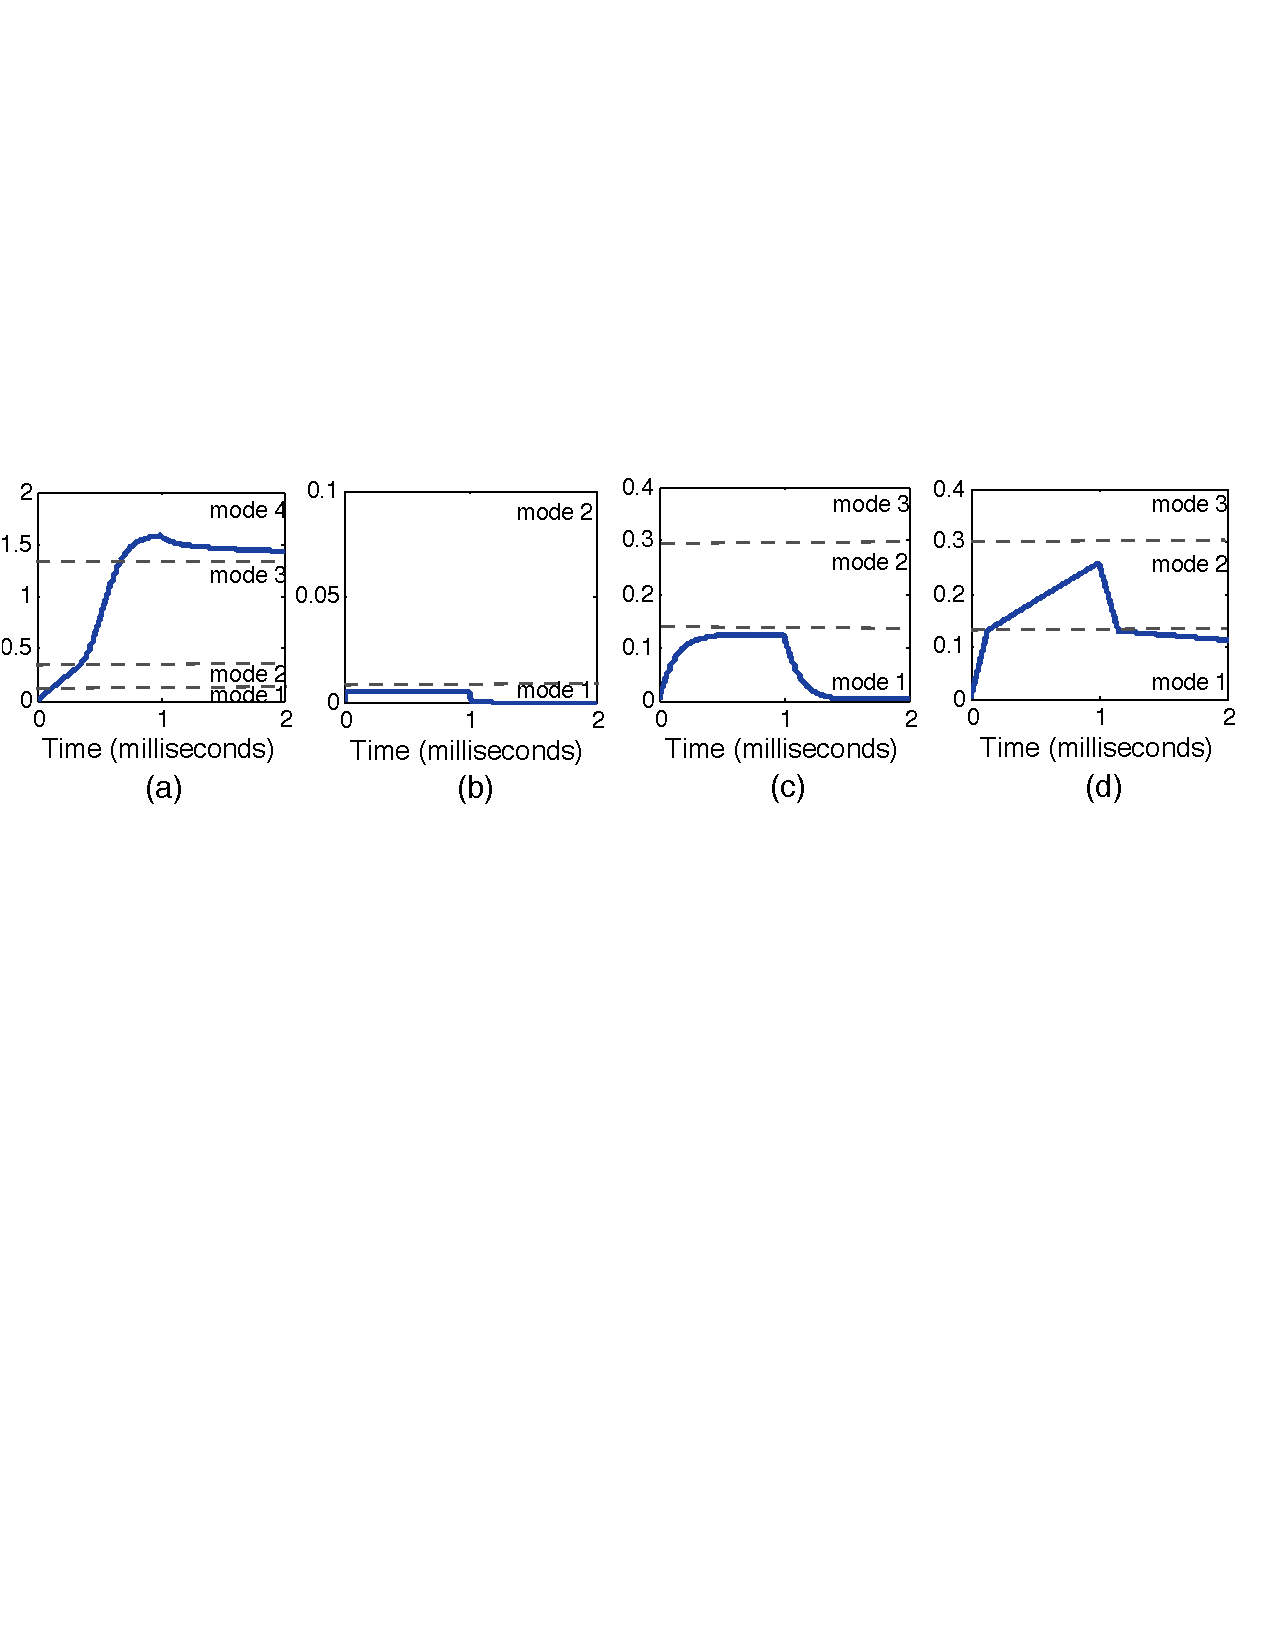
\includegraphics[scale=0.6]{fig-cardiactraj2}
\caption{Simulation results with different parameter settings. (a) Original parameters (b) $\tau_{o1}=0.0055$ (c) $\tau_{o2} = 0.125$ (d) $\tau_{so1} =1.2$, $\tau_{so2} =1.0$ }
\label{cresults}
 \vspace{-0.7cm}
\end{figure}

%\paragraph{Mode 1 (recovering resting mode)}
%The $\flow_1$ condition:
%\begin{eqnarray*}
%\frac{du}{dt}&=& \epsilon - \frac{u}{\tau_{o1}}\\
%\frac{dv}{dt}&=& \frac{1 - v}{\tau_{v1}^-}\\
%\frac{dw}{dt}&=&  \displaystyle\frac{1 -  \displaystyle\frac{u}{\tau_w^{\infty}}-w}{\tau_{w1}^{-}+(\tau_{w2}^{-}-\tau_{w1}^{-}) \displaystyle\frac{1}{1+e^{-2k_{w}^{-}(u-u_{w}^{-})}}}\\
%\frac{ds}{dt}&=& \Big(\frac{1}{1+e^{-2k_{s}(u-u_{s})}}-s\Big)\frac{1}{\tau_{s1}}
%\end{eqnarray*}
%The jump condition $\jump_{1 \rightarrow 2}: u \geq \theta_o$
%
%\paragraph{Mode 2 (recovering resting mode)}
%The $\flow_2$ condition:
%\begin{eqnarray*}
%\frac{du}{dt}&=& \epsilon - \frac{u}{\tau_{o2}}\\
%\frac{dv}{dt}&=& \frac{- v}{\tau_{v2}^-}\\
%\frac{dw}{dt}&=&  \displaystyle\frac{w_{\infty}^{*}  -  w}{\tau_{w1}^{-}+(\tau_{w2}^{-}-\tau_{w1}^{-}) \displaystyle\frac{1}{1+e^{-2k_{w}^{-}(u-u_{w}^{-})}}}\\
%\frac{ds}{dt}&=& \Big(\frac{1}{1+e^{-2k_{s}(u-u_{s})}}-s\Big)\frac{1}{\tau_{s1}}
%\end{eqnarray*}
%The jump condition $\jump_{2 \rightarrow 1}: u < \theta_o$, $\jump_{2 \rightarrow 3}: u \geq \theta_w$
%
%\paragraph{Mode 3 (recovering resting mode)}
%The $\flow_3$ condition:
%\begin{eqnarray*}
%\frac{du}{dt}&=& \epsilon - \displaystyle\frac{1}{\tau_{so1}+(\tau_{so2}-\tau_{so1})\displaystyle\frac{1}{1+e^{-2k_{so}(u-u_{so})}}}+w\frac{s}{\tau_{si}}\\
%\frac{dv}{dt}&=& \frac{- v}{\tau_{v2}^-}\\
%\frac{dw}{dt}&=&  \frac{-w}{\tau_w^+}\\
%\frac{ds}{dt}&=& \Big(\frac{1}{1+e^{-2k_{s}(u-u_{s})}}-s\Big)\frac{1}{\tau_{s1}}
%\end{eqnarray*}
%The jump condition $\jump_{3 \rightarrow 2}: u < \theta_w$, $\jump_{3 \rightarrow 4}: u \geq \theta_v$
%
%
%\paragraph{Mode 4 (recovering resting mode)}
%The $\flow_4$ condition:
%\begin{eqnarray*}
%\frac{du}{dt}&=& \epsilon + v (u-\theta_v)(u_u-u) \frac{1}{\tau_{fi}}\\
%                    &  &  - \displaystyle\frac{1}{\tau_{so1}+(\tau_{so2}-\tau_{so1})\displaystyle\frac{1}{1+e^{-2k_{so}(u-u_{so})}}}+w\frac{s}{\tau_{si}}\\
%\frac{dv}{dt}&=& \frac{- v}{\tau_{v2}^+}\\
%\frac{dw}{dt}&=&  \frac{-w}{\tau_w^+}\\
%\frac{ds}{dt}&=& \Big(\frac{1}{1+e^{-2k_{s}(u-u_{s})}}-s\Big)\frac{1}{\tau_{s2}}
%\end{eqnarray*}
%The jump condition $\jump_{3 \rightarrow 2}: u < \theta_v$.






%\subsection{EGF-NGF signaling pathway model}

%PC12 cells are a valuable model system in neuroscience. They proliferate in response to EGF stimulation but differentiate into sympathetic neurons in response to NGF. This interesting phenomenon has been intensively studied \citep{brown}. It has been reported that the signal specificity is correlated with different Erk dynamics. Specifically, a transient activation of Erk1/2 has been associated with cell proliferation, while a sustained activity has been linked to differentiation. How EGF and NGF affect the dynamics of active Erk through a network of intermediate signaling proteins is shown schematically in Figure 2. This model not only includes a common pathway to Erk through Ras shared by both the EGFR and NGFR, but also includes two important side branches through PI3K and C3G, which introduce multiple feedback loops thus complicating the dynamics. The ODE model of this pathway is available in the BioModels database \citep{}. It consists of 32 differential equations and 48 associated rate parameters (estimated from multiple sets of experimental data).


%\begin{figure}
%\centering
%\includegraphics[scale=0.3]{EGFNGF2.pdf}
%\caption{EGF-NGF pathway}
%\label{egf-ngf}
%\end{figure}


%This case study is for parameter estimation. Our advantage is that we can estimate interval values for parameters using noisy experimental data (i.e. data points with error bars). it implies that our method takes account of the stochasticity of bio-systems and can identify a robust region of the parameter solution space.

%We translate an ODE model into a hybrid model using the experimental data and then check if it can reach the final mode.
%the expected result is:
%egfngf: sat, with parameter intervals
%In Figure ?, we show the fitting graphs, i.e. trajectories generated using the estimated parameters fit the data.

% END




%The model has two modes which are defined as follows:

%\paragraph{Mode 1 (on-treatment)}
%The $\flow_1$ condition:
%\begin{eqnarray*}
%\frac{dx}{dt}&=& \Big(\alpha_x \Big(k_1+(1-k_1)\frac{z}{z+k_2}\Big)-\beta_x\Big(k_3+(1-k_3)\frac{z}{z+k_4}\Big)\\
%                    &  & - m_1\Big(1-\frac{z}{z_0}\Big)\Big)x\\
%\frac{dy}{dt}&=& m_1\Big(1-\frac{z}{z_0}\Big)+\alpha_y \Big(1- d\frac{z}{z_0}\Big) - \beta_y\\
%\frac{dz}{dt}&=& \frac{-z}{\tau}
%\end{eqnarray*}
%The jump condition $\jump_{1 \rightarrow 2}:$
%$$x + y \leq r_0 \wedge \frac{dx}{dt} + \frac{dy}{dt} < 0$$
%
%\paragraph{Mode 2 (off-treatment)}
%The $\flow_2$ condition:
%\begin{eqnarray*}
%\frac{dx}{dt}&=& \Big(\alpha_x \Big(k_1+(1-k_1)\frac{z}{z+k_2}\Big)-\beta_x\Big(k_3+(1-k_3)\frac{z}{z+k_4}\Big)\\
%                    &  & - m_1\Big(1-\frac{z}{z_0}\Big)\Big)x\\
%\frac{dy}{dt}&=& m_1\Big(1-\frac{z}{z_0}\Big)+\alpha_y \Big(1- d\frac{z}{z_0}\Big) - \beta_y\\
%\frac{dz}{dt} &=& \frac{z_0-z}{\tau}
%\end{eqnarray*}
%The jump condition $\jump_{2 \rightarrow 1}:$
%$$x + y \geq r_1 \wedge \frac{dx}{dt} + \frac{dy}{dt} > 0$$
%where $x(t)$, $y(t)$, and $z(t)$ represent the population of AD cells, the population of AI cells, and the serum androgen concentration, respectively. The growth dynamics of AD and AI cells are governed by their proliferation rate, apoptosis rate and mutation rate from AD to AI phenotype, depending on androgen concentration $z(t)$. The PSA level $v$ (ng ml$^{-1}$) is defined as $v(t)=x(t)+y(t)$. The treatment is suspended or restarted according to the value of $v$ and ${dv}/{dt}$. In mode $2$ (off-treatment), the androgen concentration is maintained at the normal level $z_0$ by homeostasis. In mode $1$ (on-treatment), the androgen is cleared at a rate $1/\tau$. Table \ref{prostate} lists the values of model parameters.




%The model is defined as follows:
%\paragraph{Mode 1 (on-treatment)}
%The $\flow_1$ condition:
%\begin{eqnarray*}
%\frac{dx}{dt} &=& (G_x(z) - M_{xy}(z))x\\
%\frac{dy}{dt} &=& M_{xy}(z)x+G_y(z)y\\
%\frac{dz}{dt} &=& \frac{-z}{\tau}
%\end{eqnarray*}
%The jump condition $\jump_{1 \rightarrow 2}:$
%$$x + y \leq r_0 \wedge \frac{dx}{dt} + \frac{dy}{dt} < 0$$
%
%\paragraph{Mode 2 (off-treatment)}
%The $\flow_2$ condition:
%\begin{eqnarray*}
%dx/dt &=& (G_x(z) - M_{xy}(z))x\\
%dy/dt &=& M_{xy}(z)x+G_y(z)y\\
%dz/dt &=& \frac{z_0-z}{\tau}
%\end{eqnarray*}
%The jump condition $\jump_{2 \rightarrow 1}:$
%$$x + y \geq r_1 \wedge \frac{dx}{dt} + \frac{dy}{dt} > 0$$
%where $x$, $y$, and $z$ represent the population of androgen dependent (AD) cells, the population of androgen independent (AI) cells, and androgen concentration, respectively. The PSA level $v$ (ng ml$^{-1}$)is defined as $v=x+y$. The treatment is suspended or restarted according to the value of $v$ and $\fact{dv}{dt}$. The growth of AD cells and AI cells are governed by the respective net growth rates $G_x{z}$ and $G_y(z)$ and the mutation rate $M_{xy}{z}$ from the AD to AI phenotype. Theses are represented as follows:
%\begin{eqnarray*}
%G_x(z) &=& \alpha_x
%(k_1+(1-k_1)\frac{z}{z+k_2})-\beta_x(k_3+(1-k_3)\frac{z}{z+k_4})\\
%G_y(z) &=& \alpha_y (1- d\frac{z}{z_0}) - \beta_y\\
%M_{xy}(z) &=& m_1(1-\frac{z}{z_0})
%\end{eqnarray*}





